\documentclass[11pt,a4paper]{article}
\usepackage[utf8]{inputenc}
\usepackage[french]{babel}
\usepackage[T1]{fontenc}

\usepackage{amsmath}
\usepackage{amsfonts}
\usepackage{amssymb}

\newcommand{\NomAuteur}{Fabrice BOISSIER}
\newcommand{\TitreMatiere}{Algorithmique 1}
\newcommand{\NomUniv}{EPITA - Bachelor Cyber Sécurité}
\newcommand{\NiveauUniv}{CYBER1}
\newcommand{\NumGroupe}{CYBER1}
\newcommand{\AnneeUniv}{2024-2025}
\newcommand{\DateExam}{27 janvier 2025}
\newcommand{\TypeExam}{Partiel (Sujet A) CORRECTION}
\newcommand{\TitreExam}{\TitreMatiere}
\newcommand{\DureeExam}{2h00}
\newcommand{\MyWaterMark}{\AnneeUniv} % Watermark de protection

% Ajout de mes classes & definitions
\usepackage{MetalExam} % Appelle un .sty

% "Tableau" et pas "Table"
\addto\captionsfrench{\def\tablename{Tableau}}

%%%%%%%%%%%%%%%%%%%%%%%
%Header
%%%%%%%%%%%%%%%%%%%%%%%
\lhead{\TypeExam}							%Gauche Haut
\chead{\NomUniv}							%Centre Haut
\rhead{\NumGroupe}							%Droite Haut
\lfoot{\DateExam}							%Gauche Bas
\cfoot{\thepage{} / \pageref*{LastPage}}	%Centre Bas
\rfoot{\texttt{\TitreMatiere}}				%Droite Bas

%%%%%

\usepackage{tabularx}

\newlength{\LabelWidth}%
%\setlength{\LabelWidth}{1.3in}%
\setlength{\LabelWidth}{1cm}%
%\settowidth{\LabelWidth}{Employee E-mail:}%  Specify the widest text here.

% Optional first parameter here specifies the alignment of
% the text within the \makebox.  Default is [l] for left
% alignment. Other options are [r] and [c] for right and center
\newcommand*{\AdjustSize}[2][l]{\makebox[\LabelWidth][#1]{#2}}%


\definecolor{mGreen}{rgb}{0,0.6,0}
\definecolor{mGray}{rgb}{0.5,0.5,0.5}
\definecolor{mPurple}{rgb}{0.58,0,0.82}
\definecolor{backgroundColour}{rgb}{0.95,0.95,0.92}

\lstdefinestyle{CStyle}{
    backgroundcolor=\color{backgroundColour},
    commentstyle=\color{mGreen},
    keywordstyle=\color{magenta},
    numberstyle=\tiny\color{mGray},
    stringstyle=\color{mPurple},
    basicstyle=\footnotesize,
    breakatwhitespace=false,
    breaklines=true,
    captionpos=b,
    keepspaces=true,
    numbers=left,
    numbersep=5pt,
    showspaces=false,
    showstringspaces=false,
    showtabs=false,
    tabsize=2,
    language=C
}


\hyphenation{op-tical net-works SIGKILL}


\begin{document}

\MakeExamTitleDuree              % Pour afficher la duree
%\MakeExamTitle                   % Ne pas afficher la duree

%% \MakeStudentName    %% A reutiliser sur chaque nouvelle page

\bigskip
%\bigskip

\noindent Vous devez respecter les consignes suivantes, sous peine de 0 :

\begin{itemize}
\item Lisez le sujet en entier avec attention
\item Répondez sur le sujet
\item Ne détachez pas les agrafes du sujet
\item \'Ecrivez lisiblement vos réponses (si nécessaire en majuscules)
%\item Vous devez écrire dans le langage algorithmique ou en C (donc pas de Python ou autre)
\item \'Ecrivez lisiblement votre nom et votre prénom sur la copie \newline
       dans les champs prévus au dessus de cette consigne
\item Ne trichez pas
\end{itemize}

%\bigskip

%%%%%%%%%%%%%%%%% CENTRAGE
\vfillFirst

% Questions cours
\section{Questions (sur 6 points)}

%\bigskip

\subsection{(3 points) En admettant que l'on dispose d'une pile vide et que les éléments \og 1 2 3 4 5 6 \fg{} arrivent en entrée dans cet ordre exclusivement, et qu'à chaque fois qu'un élément est sorti, celui-ci est affiché, décrivez les scénarios permettant d'obtenir les sorties suivantes : }

%\bigskip

\begin{center}
\noindent \textit{exemple : pour \og A B C \fg{} en entrée, on peut obtenir \og B C A \fg{} en sortie en faisant : \linebreak
\og push A \fg, \og push B \fg, \og pop \fg, \og push C \fg, \og pop \fg, \og pop \fg }
%%% AJOUTER CE TEXTE :
%On a bien inséré A, puis B, puis C, mais l'ordre de sortie est différent suivant les \og pop \fg}
\end{center}

%\medskip


\begin{center}
\begin{table}[ht!]
  \centering
  \begin{minipage}{0.33\textwidth}

\begin{center}
\begin{large}
3, 2, 4, 1, 6, 5
\end{large}

\medskip

%\GrilleReponseXY{5}{11.0}
% push 1, push 2, push 3, pop, pop, push 4, pop, pop, push 5, push 6, pop, pop
\begin{itemize}
\item Push 1
\item Push 2
\item Push 3
\item Pop
\item Pop
\item Push 4
\item Pop
\item Pop
\item Push 5
\item Push 6
\item Pop
\item Pop
\end{itemize}

\end{center}

  \end{minipage}
  \hfillx
  \begin{minipage}{0.33\textwidth}

\begin{center}
\begin{large}
2, 3, 1, 4, 6, 5
\end{large}

\medskip

%\GrilleReponseXY{5}{11.0}
% push 1, push 2, pop, push 3, pop, pop, push 4, pop, push 5, push 6, pop, pop
\begin{itemize}
\item Push 1
\item Push 2
\item Pop
\item Push 3
\item Pop
\item Pop
\item Push 4
\item Pop
\item Push 5
\item Push 6
\item Pop
\item Pop
\end{itemize}

\end{center}

  \end{minipage}
  \hfillx
  \begin{minipage}{0.33\textwidth}

\begin{center}
\begin{large}
1, 4, 3, 2, 5, 6
\end{large}

\medskip

%\GrilleReponseXY{5}{11.0}
% push 1, pop, push 2, push 3, push 4, pop, pop, pop, push 5, pop, push 6, pop
\begin{itemize}
\item Push 1
\item Pop
\item Push 2
\item Push 3
\item Push 4
\item Pop
\item Pop
\item Pop
\item Push 5
\item Pop
\item Push 6
\item Pop
\end{itemize}

\end{center}

  \end{minipage}
\end{table}
\end{center}



\vfillLast
%%%%%%%%%%%%%%%%% CENTRAGE

\clearpage

%%%%%%%%%%%%%%%%%%%%%%%%%%%%%

\subsection{(1 point) Donnez les caractéristiques de cette file dans chaque principe de fonctionnement : }

\begin{center}
\textit{Le but de l'exercice est d'illustrer les différences produites entre les 2 principales logiques d'implémentation des files}
\end{center}

%\bigskip

\begin{figure}[ht!]
\centering
\centerline{  %%% CENTRAGE HORIZONTAL
%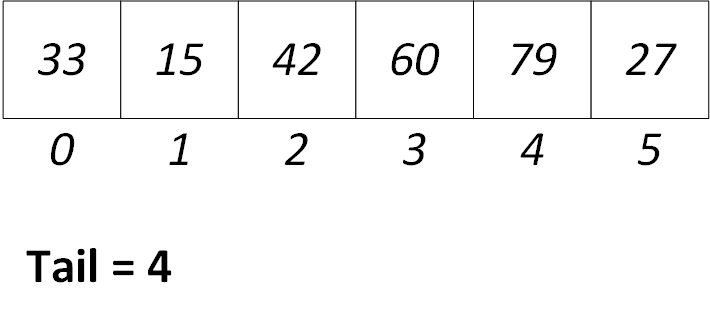
\includegraphics[height=3.5cm]{img/file_t_1_A.png}
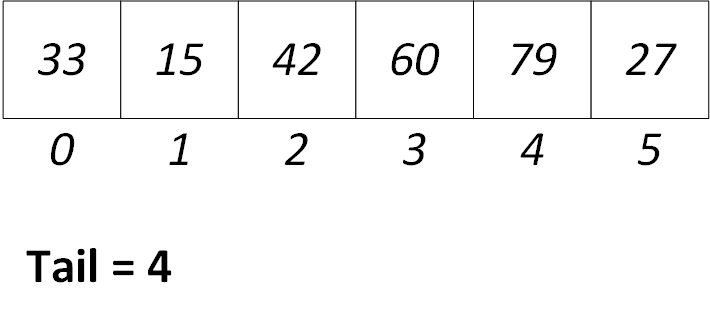
\includegraphics[height=3.0cm]{img/file_t_1_A.png}
%\includegraphics[height=1.85cm]{img/file_t_1.png}
%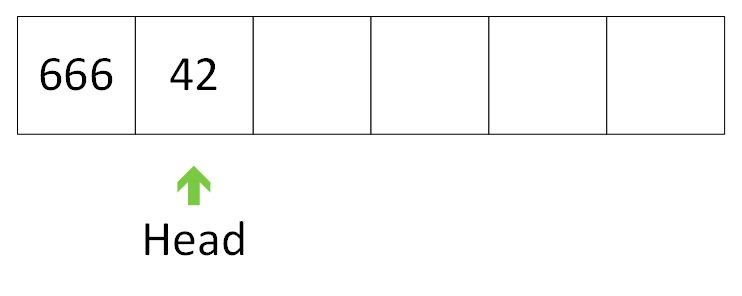
\includegraphics[scale=1,left]{img/2_elts.png}
}
\end{figure}

%\medskip
\vspace*{-0.5cm}

\begin{center}
En admettant que la queue de la file (Tail) est initialisée à la case \og -1 \fg{} lorsqu'elle est vide, indiquez :

\begin{table}[ht!]
  \centering
  \begin{minipage}{0.4\textwidth}

\textbf{Taille maximale de la file :  \hspace*{0.25cm }  6}

\bigskip
%\vspace*{1.5cm}

\textbf{Longueur utilisée de la file :  \hspace*{0.25cm }  5}

  \end{minipage}
  \hfillx
  \begin{minipage}{0.6\textwidth}

\textbf{\'Elément qui sera effacé lors du prochain \textit{enqueue} :    27}

\bigskip
%\vspace*{1.5cm}

\textbf{Prochain élément défilé :  \hspace*{0.25cm }  33}

  \end{minipage}
\end{table}


%\bigskip
\vspace*{1cm}

%%%%%%%%%%%%%%%

En admettant que la queue de la file (Tail) est initialisée à la case \og 0 \fg{} lorsqu'elle est vide, indiquez :

\begin{table}[ht!]
  \centering
  \begin{minipage}{0.4\textwidth}

\textbf{Taille maximale de la file :  \hspace*{0.25cm }  6}

\bigskip
%\vspace*{1.5cm}

\textbf{Longueur utilisée de la file :  \hspace*{0.25cm }  4}

  \end{minipage}
  \hfillx
  \begin{minipage}{0.6\textwidth}

\textbf{\'Elément qui sera effacé lors du prochain \textit{enqueue} :    79}

\bigskip
%\vspace*{1.5cm}

\textbf{Prochain élément défilé :  \hspace*{0.25cm }  33}

  \end{minipage}
\end{table}
\end{center}


\bigskip



\bigskip
\bigskip

%%%%%%%%%%%%%%%%%%%%%%%%%%%%%

\subsection{(2 points) Donnez l'état final des tableaux sous-jacents aux structures de données vues en cours suite aux appels successifs suivants : }


\begin{center}
\begin{table}[ht!]
  \centering
  \begin{minipage}{0.45\textwidth}

% Push D, Push A, Push B, Pop, Push C, Pop, Push N, Push B, Pop, Pop, Push N, Push C, Push F, Pop, Push E

\begin{center}
\begin{tabular}{c L{2cm} L{2cm} L{2cm} c }
$\Rightarrow$ & Push D, & Push A, & Push B,  & \phantom{Iq} \\
& Pop,    & Push C, & Pop,     & \phantom{Iq} \\
& Push N, & Push B, & Pop,     & \phantom{Iq} \\
& Pop,    & Push N, & Push C,  & \phantom{Iq} \\
& Push F, & Pop,    & Push E. $\Rightarrow$ & \phantom{Iq} \\
\end{tabular}
\end{center}

  \end{minipage}
  \hfillx
  \begin{minipage}{0.01\textwidth}

\begin{tikzpicture}
\draw (0,0) -- (0,3.0);
\end{tikzpicture}

  \end{minipage}
  \hfillx
  \begin{minipage}{0.45\textwidth}

% Enqueue D, Enqueue U, Enqueue B, Dequeue, Enqueue D, Enqueue I, Enqueue N, Dequeue, Dequeue, Enqueue O

\begin{center}
\begin{tabular}{c L{2.5cm} L{2.5cm} c }
$\Rightarrow$
& Enqueue D, & Enqueue U,  & \phantom{Iq} \\
& Enqueue B, & Dequeue,    & \phantom{Iq} \\
& Enqueue D, & Enqueue I,  & \phantom{Iq} \\
& Enqueue N, & Dequeue,    & \phantom{Iq} \\
& Dequeue,   & Enqueue O. $\Rightarrow$ & \phantom{Iq} \\
\end{tabular}
\end{center}

  \end{minipage}
\end{table}
\end{center}



\begin{center}
\begin{table}[ht!]
  \centering
  \begin{minipage}{0.45\textwidth}

\begin{center}
\begin{tabular}{ |C{1.1cm}|C{1.1cm}|C{1.1cm}|C{1.1cm}|C{1.1cm}| }
\hline
\multirow{3}{*}{D} & \multirow{3}{*}{A} & \multirow{3}{*}{N} & \multirow{3}{*}{C} & \multirow{3}{*}{E} \\
%\phantom{42} & \phantom{42} & \phantom{42} & \phantom{42} & \phantom{42} \\
 & & & & \\
 & & & & \\
\hline
\end{tabular}
%
\begin{tabular}{ C{1.1cm} C{1.1cm} C{1.1cm} C{1.1cm} C{1.1cm} }
\textit{0} & \textit{1} & \textit{2} & \textit{3} & \textit{4} \\
\end{tabular}
\end{center}

  \end{minipage}
  \hfillx
  \begin{minipage}{0.01\textwidth}

\phantom{i}

  \end{minipage}
  \hfillx
  \begin{minipage}{0.45\textwidth}

\begin{center}
\begin{tabular}{ |C{1.1cm}|C{1.1cm}|C{1.1cm}|C{1.1cm}|C{1.1cm}| }
\hline
\multirow{3}{*}{D} & \multirow{3}{*}{I} & \multirow{3}{*}{N} & \multirow{3}{*}{O} & \multirow{3}{*}{\textit{(O)}} \\
%\phantom{42} & \phantom{42} & \phantom{42} & \phantom{42} & \phantom{42} \\
 & & & & \\
 & & & & \\
\hline
\end{tabular}
%
\begin{tabular}{ C{1.1cm} C{1.1cm} C{1.1cm} C{1.1cm} C{1.1cm} }
\textit{0} & \textit{1} & \textit{2} & \textit{3} & \textit{4} \\
\end{tabular}
\end{center}

  \end{minipage}
\end{table}
\end{center}



%\bigskip
\clearpage

%%%%%%%%%%%%%%%%%%%%%%%%%%%%%%%%%%%%%%%%%%%%%%%%%

\section{Algorithmes (sur 14 points)}

%\subsection{Tris}
%
%\subsubsection{(3 points) Expliquez un des algorithmes de tri de votre choix, puis écrivez son implémentation sous forme de code. }

\subsection{(3 points) Expliquez un des algorithmes de tri de votre choix, puis écrivez son implémentation sous forme de code. }

\textit{Explications : (1 points)}

\begin{center}
%\GrilleReponseN{10}
\GrilleReponseTextUp{7.0}{3.3}{\TTBF{Nom de l'algorithme de tri choisi :}}
\end{center}

%\medskip

\textit{Implémentation : (2 points)}

\begin{center}
\GrilleReponseN{14.5}
\end{center}


\clearpage

%%%%%%%%%%%%%%%%%%%%%%%%%%%%%%%%%%%%%%%%%%%%%%%%%%%%%%%%%%

\subsection{Pile (sur 7 points)}

\noindent Le but de cette partie sera de réécrire quelques fonctions essentielles permettant d'utiliser une pile.
Vous écrirez d'abord la structure en vous appuyant sur un modèle à base de tableaux, puis, vous implémenterez les fonctions avec cette structure.

\subsubsection{(1 point) \'Ecrivez une structure de données \og \textit{stack\_t} \fg{} pouvant servir de pile contenant des éléments étant des entiers positifs non-nuls. Cette pile doit obligatoirement s'appuyer sur un tableau. }

\bigskip

\begin{center}
\GrilleReponseN{8.5}
\end{center}

%%%%%%%%%%%%%%%%%%%%%%%%%%%%%

\begin{center}
\begin{table}[ht!]
  \centering
  \begin{minipage}{0.48\textwidth}

\subsubsection{(1 point) \'Ecrivez une fonction \og \textit{length} \fg{} qui détermine la taille d'une pile. }

\begin{center}
\GrilleReponseXY{8}{9.5}
\end{center}

  \end{minipage}
  \hfillx
  \begin{minipage}{0.48\textwidth}

\subsubsection{(1 point) \'Ecrivez une fonction \og \textit{is\_empty} \fg{} qui détermine si une pile est vide ou non. }

\begin{center}
\GrilleReponseXY{8}{9.5}
\end{center}

  \end{minipage}
\end{table}
\end{center}


\clearpage

%%%%%%%%%%%%%%%%%%%%%%%%%%%%%

\subsubsection{(2 points) \'Ecrivez une fonction \og \textit{push} \fg{} qui empile un élément dans une pile. }

\begin{center}
\GrilleReponseN{11.5}
\end{center}

%%%%%%%%%%%%%%%%%%%%%%%%%%%%%

\subsubsection{(2 points) \'Ecrivez une fonction \og \textit{pop} \fg{} qui dépile un élément d'une pile. }

\begin{center}
\GrilleReponseN{11.5}
\end{center}


\clearpage

%%%%%%%%%%%%%%%%%%%%%%%%%%%%%%%%%%%%%%%%%%%%%%%%%%%%%%%%%%

\subsection{File avec une liste (sur 4 points)}

%\noindent Le but de cette partie sera de réécrire quelques fonctions essentielles permettant d'utiliser une file, mais en utilisant l'API de la liste fournie ci-après.
\noindent Le but de cette partie sera d'implémenter quelques fonctions essentielles permettant d'utiliser une file.
Nous disposons déjà d'une implémentation de la structure de liste, fournie par l'API ci-dessous.
Vous utiliserez donc les fonctions de cette API pour réécrire les fonctions associées à la file.

%\bigskip
\medskip

\noindent \textbf{API Liste :}

\begin{itemize}
\item \TTBF{list\_t *CreateListT(int max\_len)} : crée une liste vide de taille maximale \textit{max\_len}
\item \TTBF{bool InsertListT(list\_t *l, int index, int elt)} : insère l'élément \textit{elt} à la position \textit{index} dans la liste \textit{l} (en poussant vers la droite les éléments existants)
\item \TTBF{bool RemoveListT(list\_t *l, int index)} : supprime l'élément en position \textit{index} de la liste \textit{l}
\item \TTBF{int LengthListT(list\_t *l)} : renvoie la taille de la liste \textit{l} (c'est-à-dire le nombre d'éléments présents)
\item \TTBF{int GetPositionListT(list\_t *l, int elt)} : renvoie l'index du premier élément \textit{elt} trouvé dans la liste \textit{l} (si l'élément n'est pas trouvé, la fonction renvoie \textit{-1})
\item \TTBF{int GetEltListT(list\_t *l, int index)} : renvoie l'élément présent en position \textit{index} dans la liste \textit{l} (si la position est incorrecte, la fonction renvoie \textit{-1})
\item \TTBF{bool IsEmptyListT(list\_t *l)} : teste si la liste \textit{l} est vide ou non
\item \TTBF{bool IsFullListT(list\_t *l)} : teste si la liste \textit{l} est pleine ou non
\item \TTBF{int ClearListT(list\_t *l)} : vide la liste \textit{l} et renvoie le nombre d'éléments supprimés
\item \TTBF{void DeleteListT(list\_t *l)} : supprime la liste \textit{l}
\end{itemize}

%\bigskip
\medskip

\subsubsection{(2 points) \'Ecrivez une fonction \og \textit{enqueue} \fg{} qui enfile un élément dans une liste utilisée comme une file. }

\begin{center}
\GrilleReponseN{13}
\end{center}


\subsubsection{(2 points) \'Ecrivez une fonction \og \textit{dequeue} \fg{} qui défile un élément d'une liste utilisée comme une file. }

\begin{center}
\GrilleReponseN{13}
\end{center}



\vfillFirst

\begin{center}
\textit{N'oubliez pas d'écrire votre nom et votre prénom sur la $1\up{\text{ère}}$ page.}
\end{center}

\vfillLast


\clearpage

%%%%%%%%%%%%%%%%%%%%%%%%%%%%%%%%%%%%%%%%%%%%%%%%%%%%%%%%

%\thispagestyle{empty}

\vfillFirst

\begin{center}

\begin{LARGE}
\textbf{CORRECTION SUJET A}

\bigskip

\textbf{\MakeUppercase{\TitreMatiere}}
\end{LARGE}

\end{center}

\vfillLast

\end{document}
